\chapter{Run conditions and Experimental setup}
\label{chap:physics}


\section{Run Group F}




%%%%%%%%%%%%%%%%%%
\section{The CLAS12 Spectrometer}
%%%%%%%%%%%%%%%%%%
The CLAS12 spectrometer is designed to operate with 11~GeV beam at an 
electron-nucleon luminosity of $\mathcal{L} = 
1\times10^{35}~$cm$^{-2}$s$^{-1}$. The baseline configuration of the CLAS12 
detector consists of the forward detector and the central detector 
packages~\cite{CD} (see Figure~\ref{fig:fd}). We use the forward detector for 
electron and photon detection. The central detector's silicon tracker and 
barrel micromegas will be removed to leave room for the BONuS12 RTPC.  

\begin{figure}
  \begin{center}
    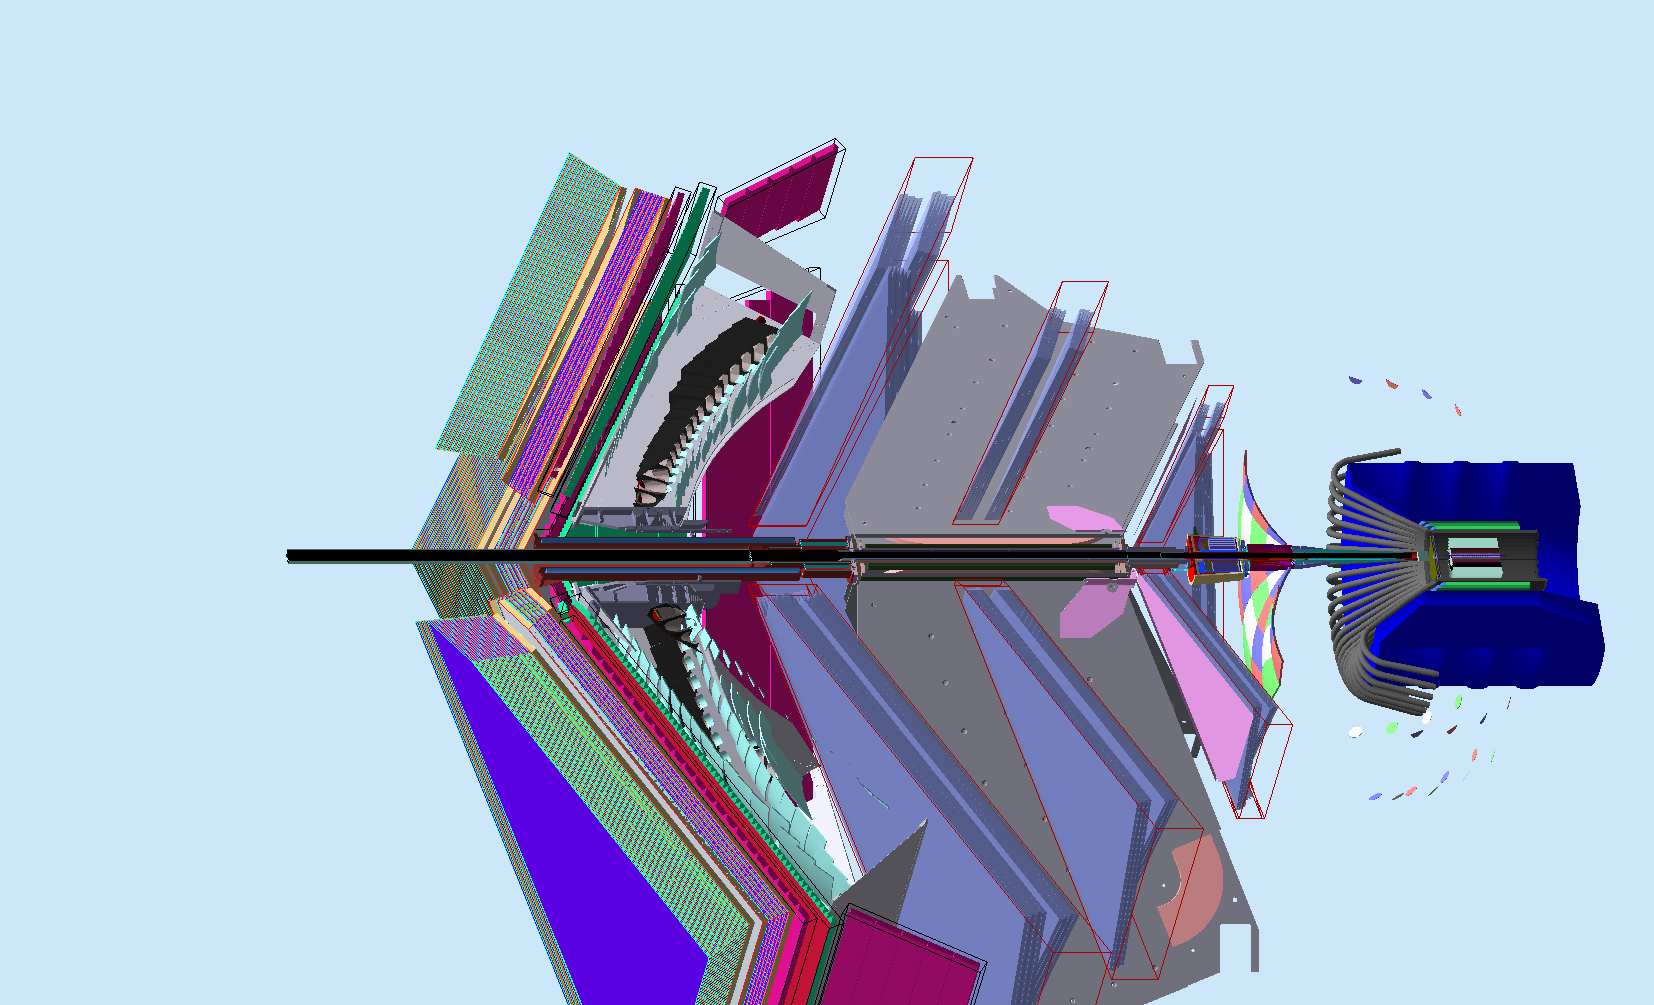
\includegraphics[angle=0, width=0.75\textwidth]{figures/clas12_bonus12.png}
     \caption{(Left) The schematic layout of the CLAS12 baseline design with 
     BONuS12 RTPC replacing the silicon tracker and the barrel micromegas.  
     (Right) Schematic layout showing BONuS12 RTPC with the modified design of 
     the forward micromegas.}
    \label{fig:fd}
  \end{center}
\end{figure}

The scattered electrons and photons will be detected in the forward detector which consists 
of the High Threshold Cherenkov Counters (HTCC), Drift Chambers (DC), the Low 
Threshold Cherenkov Counters (LTCC), the Time-of-Flight scintillators (TOF), 
the Forward Calorimeter and the Preshower Calorimeter. The charged particle 
identification in the forward detector is achieved by utilizing the combination 
of the HTCC, LTCC and TOF arrays with the tracking information from the Drift 
Chambers. The HTCC together with the Forward Calorimeter and the Preshower 
Calorimeter will provide a pion rejection factor of more than 2000 up to a 
momentum of 4.9~GeV/c, and a rejection factor of 100 above 4.9 GeV/c. The photons
are detected using the calorimeters.

